\chapter{Relevance of ATF/ATF2}
\section{Facility purpose}
The main objective of the Accelerator Test Facility (ATF) built at the High Energy Accelerator Research Organization (KEK) in Tsukuba, Japan, is to serve as R\&D platform for the requirements of linear accelerators, in particular ILC. ATF obtained the record of minimum vertical beam emittance \cite{Kubo:2001ps,PhysRevLett.92.054802}, leading to the next step, the vertical beam size reduction at the IP.\par
The Final Focus Test Beam (FFTB) \cite{Berndt:1991ug}, at the Stanford Linear Accelerator Center (SLAC) in the  U.S.A., explored the beam size reduction using the non-local chromaticity correction scheme. It operated since 1994 to 1997 with a final result of 70nm in the vertical plane. The designed 40nm was not achieved and the difference was attributed to beam jitter and tuning limitations \cite{Araki1}.\par
The beam size reduction using the local chromaticity correction is explored by an extension of the original design, called ATF2 \cite{ATF2prop,grishanov:in2p3-00309474}, then ILC-like FFS lattice scaled down to 100m with two goals: ({\textbf{goal 1}) achieve 37nm of vertical beamsize at the IP and ({\textbf{goal 2}) the stabilization of the IP beam position at the level of few nanometres.\par
The CLIC, ILC and ATF2 main parameters are shown in Table \ref{t:ILC_ATF2param}, where the vertical cromaticity $\xi_y$ is similar for ATF and ILC designs.\par
\begin{table}[hbt]
\centering
{\tiny
\begin{tabular}{l|c|c||c|c|c|c}\hline
Parameter & Symbol & Units &CLIC 3 TeV&CLIC 500 GeV& ILC & ATF2\\\hline\hline
Beam Energy per beam & $E$ & GeV & 3000 &250  &250 & 1.3 \\\hline
Energy Spread (e$^+$/e$^-$) & $\delta$ & \% & 0.3 & 0.3 & 0.07/0.12 & 0.06$\sim$0.08\\\hline
Final quad to IP distance & $L^*$ & m & 3.5 & 4.3 &3.5/4.5\dag & 1.0\\\hline
Horizontal $\beta$ function at the IP & $\beta^*_x$ & mm & 6.9 & 9 &11 & 4\\\hline
Vertical $\beta$ function at the IP & $\beta^*_y$ & mm & 0.07 & 0.2 &0.48 & 0.1\\\hline
Normalized horizontal emittance & $\epsilon^*_{xN}$ & $\mu$m & 660 & 2400 & 10 & 2.8\\\hline
Normalized vertical emittance & $\epsilon^*_{yN}$ & nm & 20 & 25 & 35 & 31\\\hline
Horizontal beam size & $\sigma^*_y$ & nm & 45 & 200 & 5.9 & 37\\\hline
Vertical beam size & $\sigma^*_y$ & nm & 0.9 & 2.3 & 5.9 & 37\\\hline
Natural vertical chromaticity & $\xi_y=L^*/\beta^*_y$ & & 50000 & 43000 &7300/9400\dag & 10000\\\hline
\end{tabular}\caption{Design parameters of ILC and ATF2 Final Focus. \dag The ILC lattice has two detector options: SiD and ILD.}\label{t:ILC_ATF2param}
}
\end{table}\par
\section{Beam line Description}
The ATF accelerator facility, shown in Fig. \ref{f:ATF}, is composed by a photocathode giving electrons to a linac which accelerates the particles to 1.3 GeV, a damping ring to reduce the beam vertical and horizontal emittance and an extraction line which provides bunch packets to the Final Focus Section (FFS) where the beam is transported to the nominal IP and dump.\par
\begin{figure}[htb]
\centering
\begin{subfigure}[b]{1.0\textwidth}
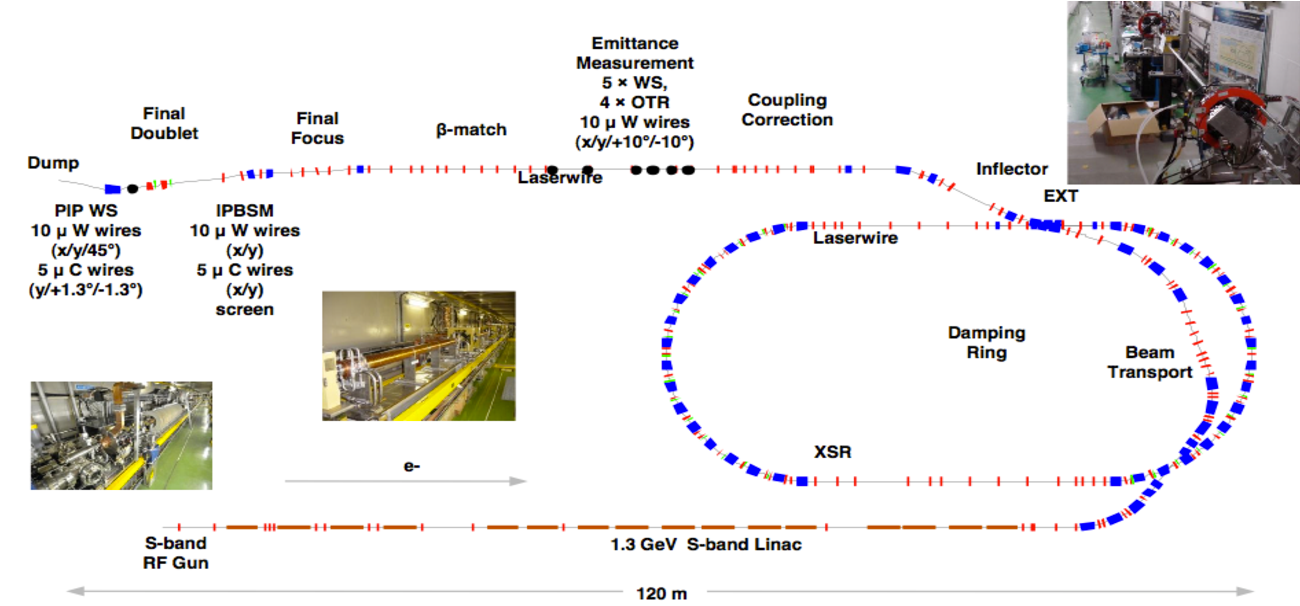
\includegraphics[angle=0,scale=0.70]{ATF-crop.pdf}\caption{Disposition of the Accelerator Test Facility (ATF), composed by a photocathode, a linac to 1.3GeV, a damping ring, an extraction line, the Final Focus (FF), and the beam dump.}\label{f:ATF_ATF2}
\end{subfigure}
\begin{subfigure}[b]{1.0\textwidth}
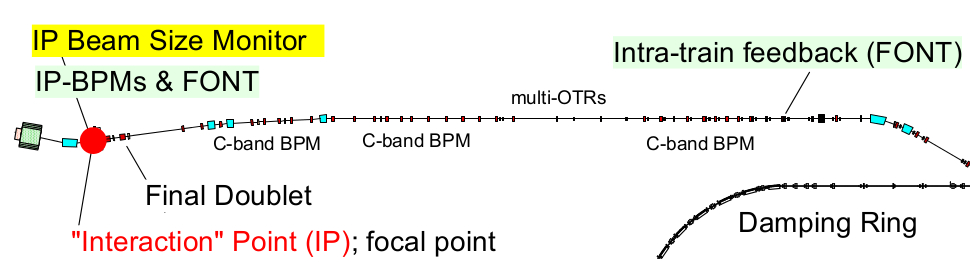
\includegraphics[angle=0,scale=0.65]{LigneATF2.jpg}\caption{Zoom over the extraction line, and Final Focus Section, highlighting the nominal Interaction Point location (IP). This region is known as ATF2.}\label{f:ATF2layout}
\end{subfigure}\caption{Diagrams containing the ATF composition and a zoom on the ATF2 section.}\label{f:ATF}
\end{figure}
The ATF2 lattice could be subdivided in two sections : the matching section and the FFS. The following section describes the FFS.\par
\subsection{The FFS}
The FFS focuses the beam to an small vertical beam size following the telescope design with local chromaticity correction, as in Sect. \ref{s:chromcorr}. The top of Fig. \ref{f:FF_MADX} shows the lattice elements and the optics functions along the FFS. The Final Doublet (FD), QD0FF and QF1FF, provide the vertical and horizontal focusing respectively. The horizontal off-momentum function $\eta$ and the pair of sextupoles in the FD is used to cancel the beam size dependence on energy spread at the IP.\par The second pair of sextupoles in the lattice section from 70 to 75 m are used to cancel the geometrical components induced by the sextupoles in the FD. And, adittional chromaticity is created upstream QF7 to match the local correction \cite{Raimondi:2000}.\par
\begin{figure}[htb]
 \vspace*{-1.5cm}
 \begin{picture}(0,0)
 \put(386,-76){\tiny IP}
 \put(372,-44){\tiny QD0}
 \put(354,-44){\tiny QF1}
 \put(198,-44){\tiny QF7}
%  \put(195,-43){\tiny IM}
%  \put(365,-76){\scriptsize FD}
 \put(70,-76){\scriptsize Matching Section}
 \put(220,-76){\scriptsize Final Focus Section (FFS)}
 \put(138,-286){\tikz\draw[blue,dashed,thick] (0,0) -- (0,8.42);}
%  \put(220,-30){\tikz\draw[red,dashed,thick] (0,0) circle (0.4);}
%  \put(-90,20){\hbar}
\end{picture}
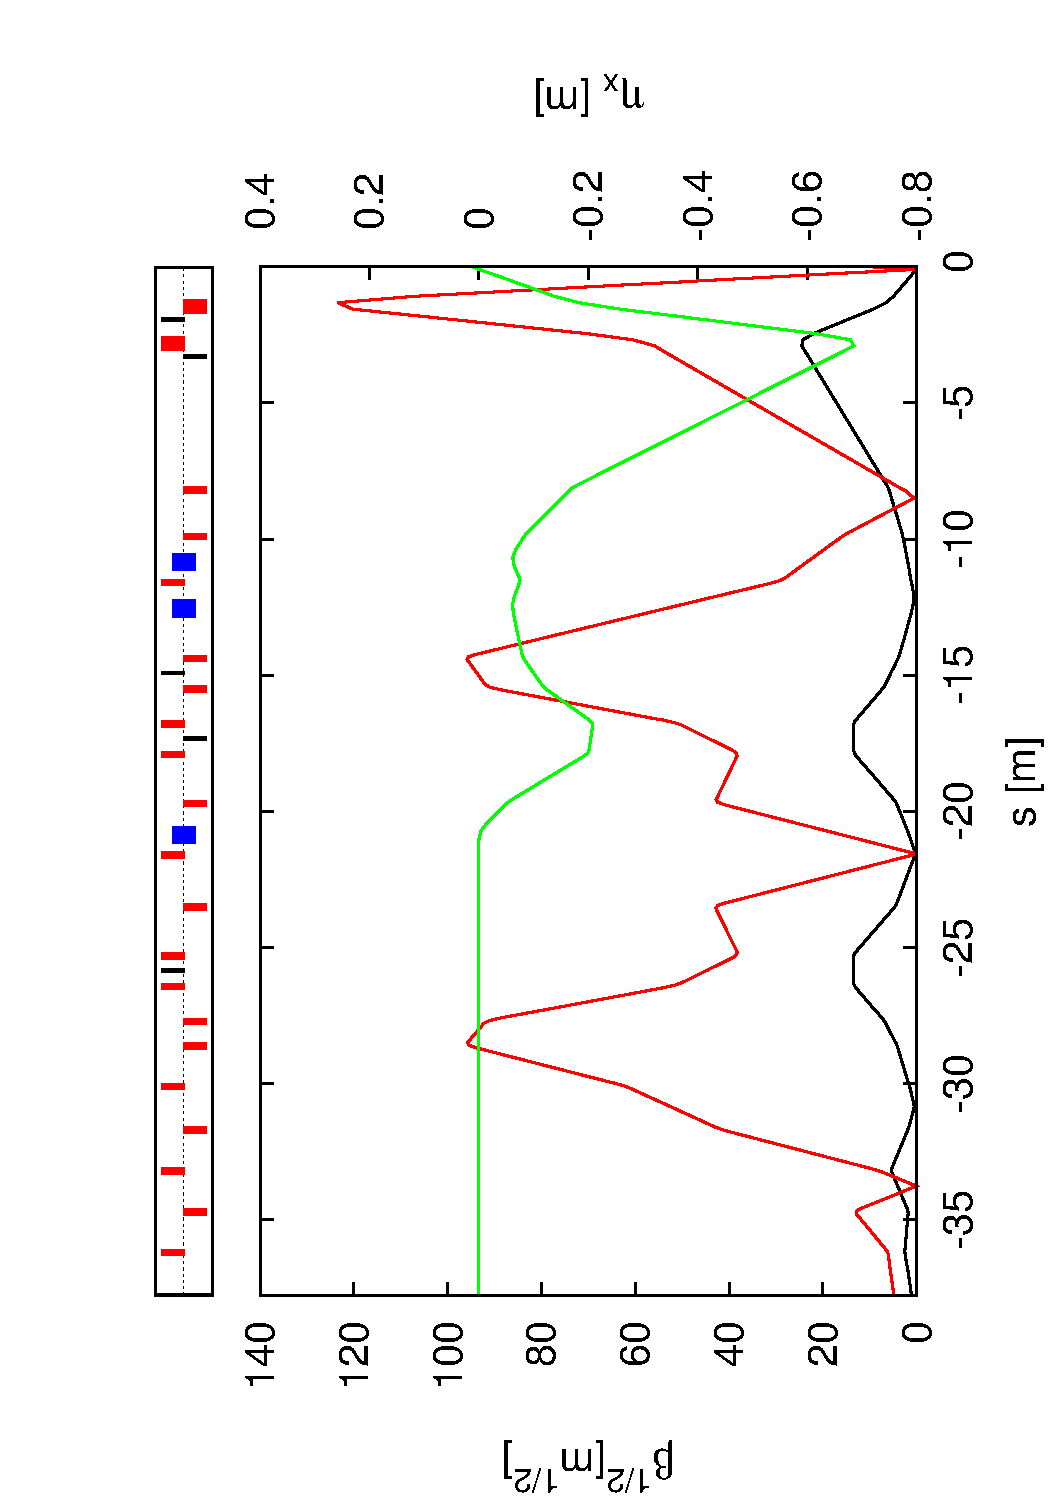
\includegraphics[angle=-90,scale=0.65]{lattice_ATF2_FF.pdf}\caption{Optical functions in the Final Focus Section at ATF2. On top is the ATF2 lattice: dipoles in blue, quadrupoles in red and sextupoles in black.}\label{f:FF_MADX}
\end{figure}
Quadrupoles displacement steers the beam, while sextupoles displacement induce focusing. This have an impact on the beam size. The tolerances to misalignments, roll angle and magnet strength errors in the FFS have been initially studied with a target of 2\% impact in the beam size, and it has shown similar tolerances results to those of ILC \cite{Yves}. 
Magnets are placed on individual movers to allow the beam steering and adjustment of relative alignment in X, Y and Roll angle. 

\subsection{Optics in the IP Region}
The $\beta^*$ functions at the IP can be set by changing the matching section magnets strength. Three configurations are normally used : 1BX1BY, 10BX1BY, and 100BX1000BY, where the factor indicates the number of times that the original $\beta^*$ has been amplified.\par
The 1BX1BY optics has the original design parameters. Here the angular divergence of the beam is $0.35$mrad vertically and $0.52$mrad horizontally in the IP region. \par
The 10BX1BY preserves the $\beta_y^*$ goal while relaxing the tolerance to multipole errors in magnets by increasing ten times the original $\beta_x^*$, making them comparable with those of ILC 500GeV \cite{PhysRevSTAB.17.023501}. This optics is the one shown in Fig. (\ref{f:FF_MADX}) and it is currently used in operation.\par
The 100BX1000BY optics sets a parallel beam through the IP area by enlarging the beam size at the IP. It is principally used to avoid the issues of large angle divergence displayed by the 1BX1BY optics.\par
Even smaller $\beta_y^*$ functions have been explored recently at ATF2 aiming to estimate lower $\beta^*$ tunability and beam size measurements limitations \cite{PateckiLowBeta}.\par
Figure (\ref{f:BXYoptics}) shows the beam size in vertical and horizontal plane for several optics combinations in a region of 300 mm around the IP. It also shows clearly how the beam divergence affects the beam size along the IP region.\par 
\begin{figure}[htb]
 \begin{center}
 \hspace*{-1cm}
 \begin{subfigure}[b]{0.45\textwidth}
  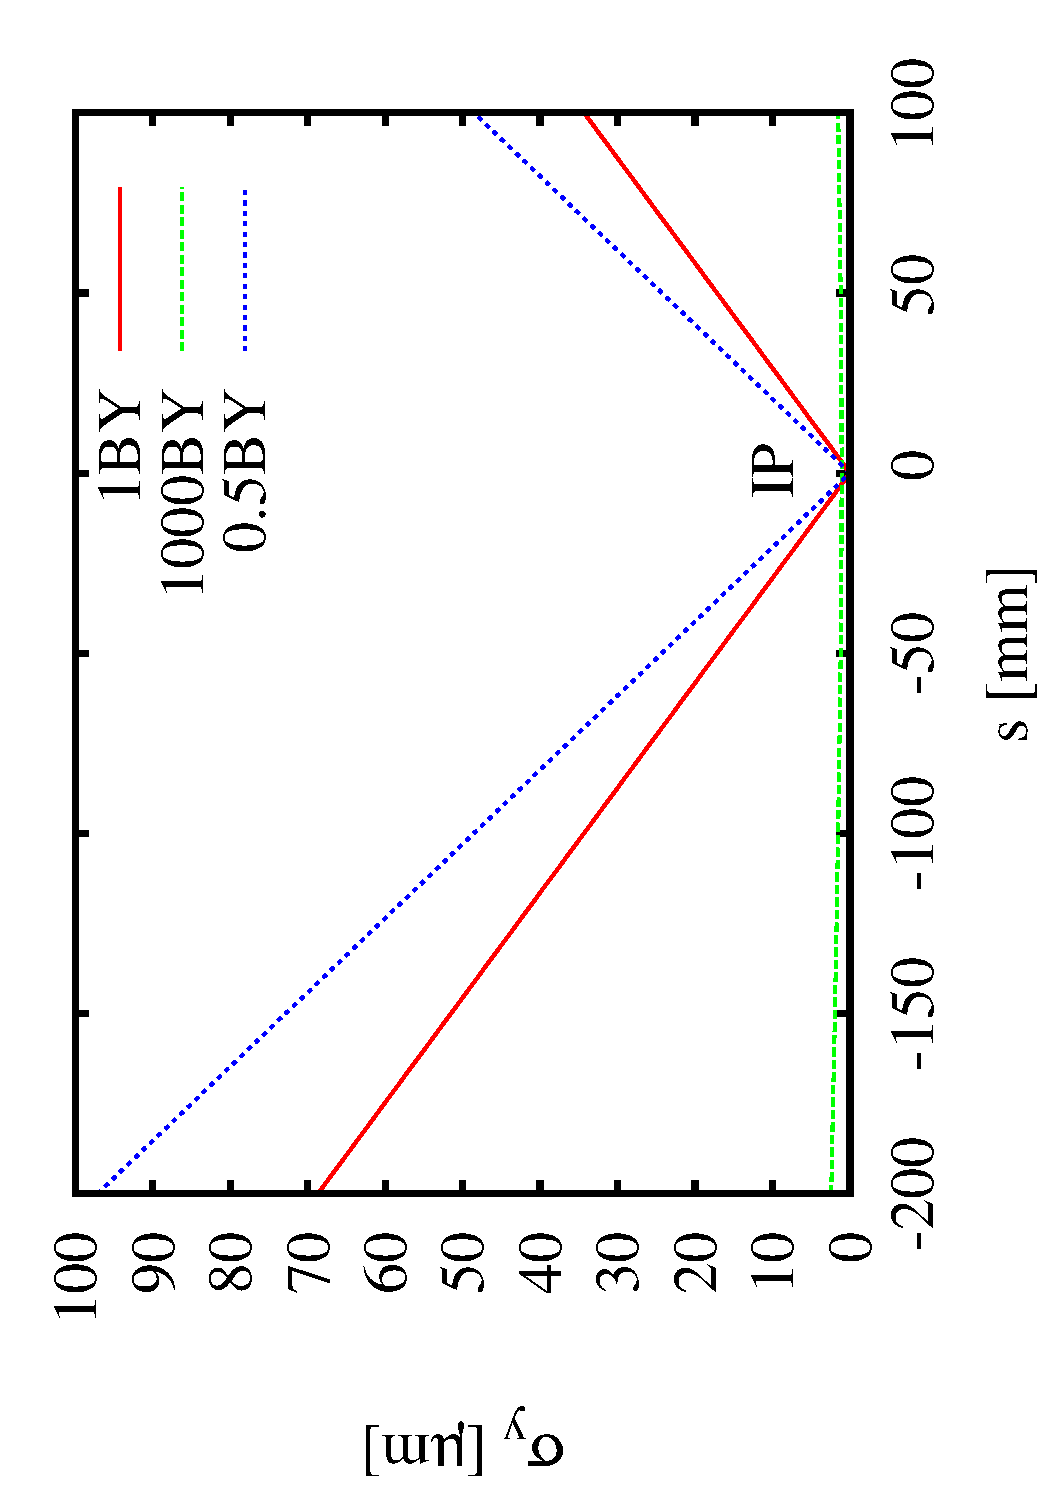
\includegraphics[angle=-90,scale=0.32]{optics_requ.pdf}\caption{Vertical beam size near the IP.}\label{f:opticsBY}
 \end{subfigure}\hspace{0.5cm}
\begin{subfigure}[b]{0.45\textwidth}
  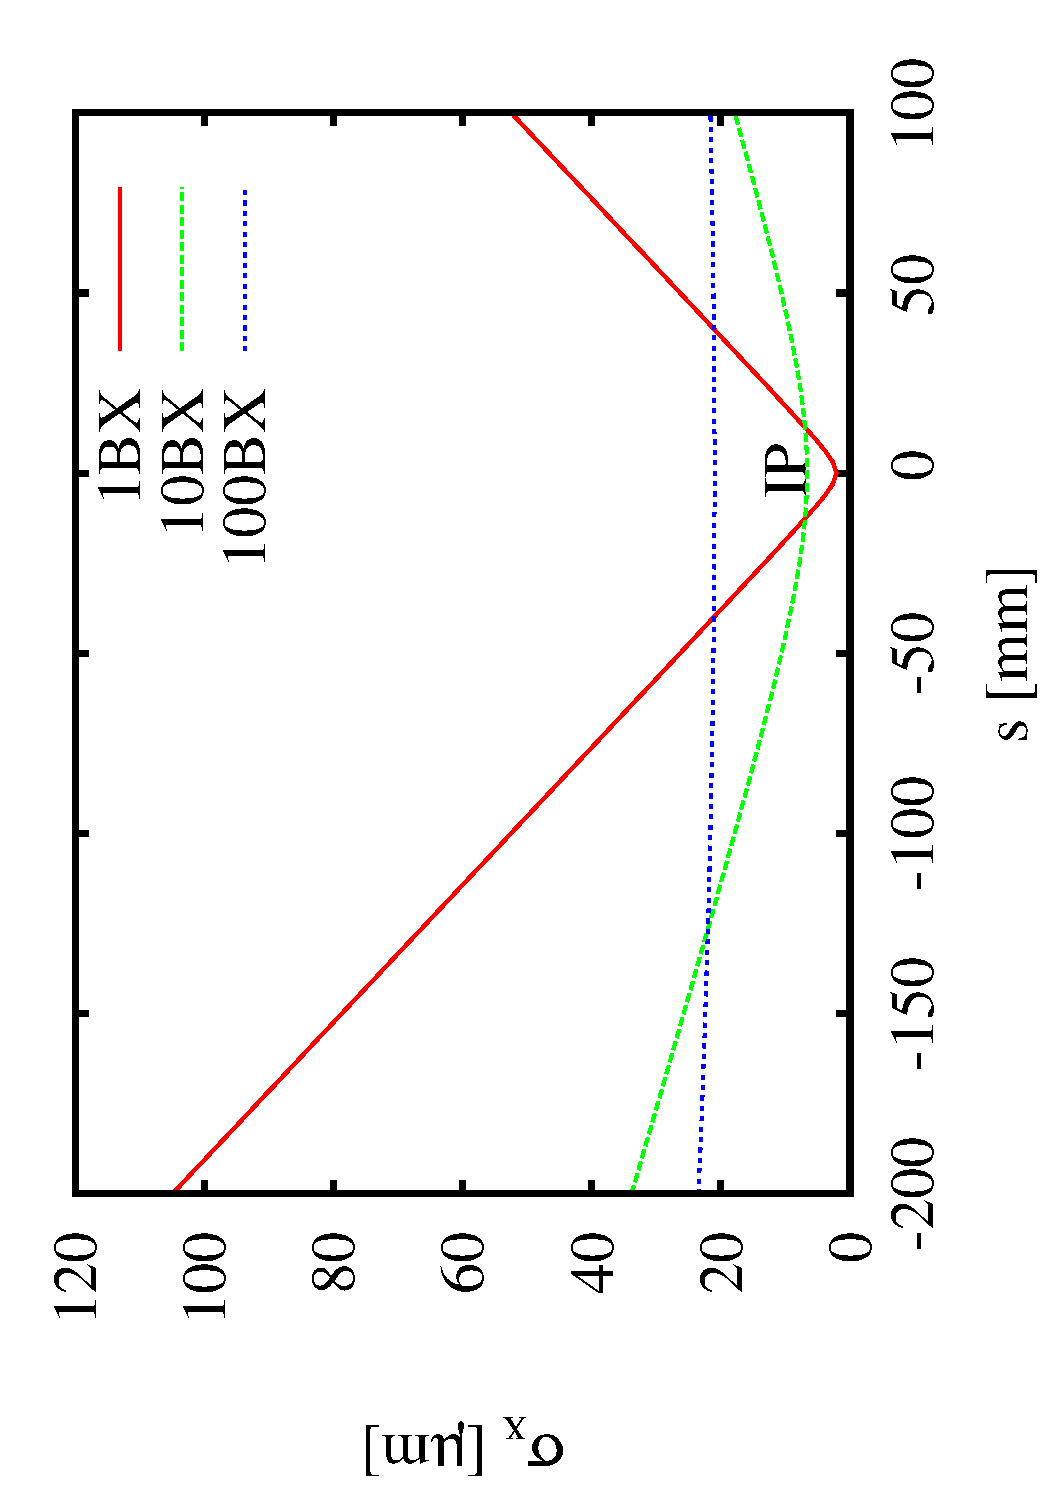
\includegraphics[angle=-90,scale=0.32]{optics_BX.pdf}\caption{Horizontal beam size near the IP.}\label{f:opticsBX}
 \end{subfigure}
  \caption{Vertical and horizontal beam sizes for 1BY, 1000BY, and 0.5BY in the vertical plane, and 1BX, 10BX and 100BX in the horizontal plane.}\label{f:BXYoptics}
 \end{center}
\end{figure}
It has been shown by upstream measurements that beam jitter upstream the FD is around 10$\sim$20\% of beam size on the vertical plane and 5$\sim$10\% on the horizontal plane \cite{PateckiJitter}.
\subsection{Beam Size Measurement at the IP (IPBSM)}
A direct beam size measurement at the ATF2 IP is required because it can not be deduced from beam-beam interaction as in any collider.\par
The Beam Size Monitor (IPBSM) at the ATF2 IP measures the number of scattered photons from an electron-photon collission between the particle bunch and a perpendicular interference pattern generated by high intensity laser perpendicular to the bunch trajectory \cite{Shintake1992453}. The number of photons is proportional to the photon density at the beam position. Moving the beam or scanning the phase of the laser fringe produces a modulation of gamma flux ray depending on beam size \cite{Yves}. Figure \ref{f:IPBSM} shows an schematic design of the IPBSM.\par
\begin{figure}[htb]
 \begin{center}
  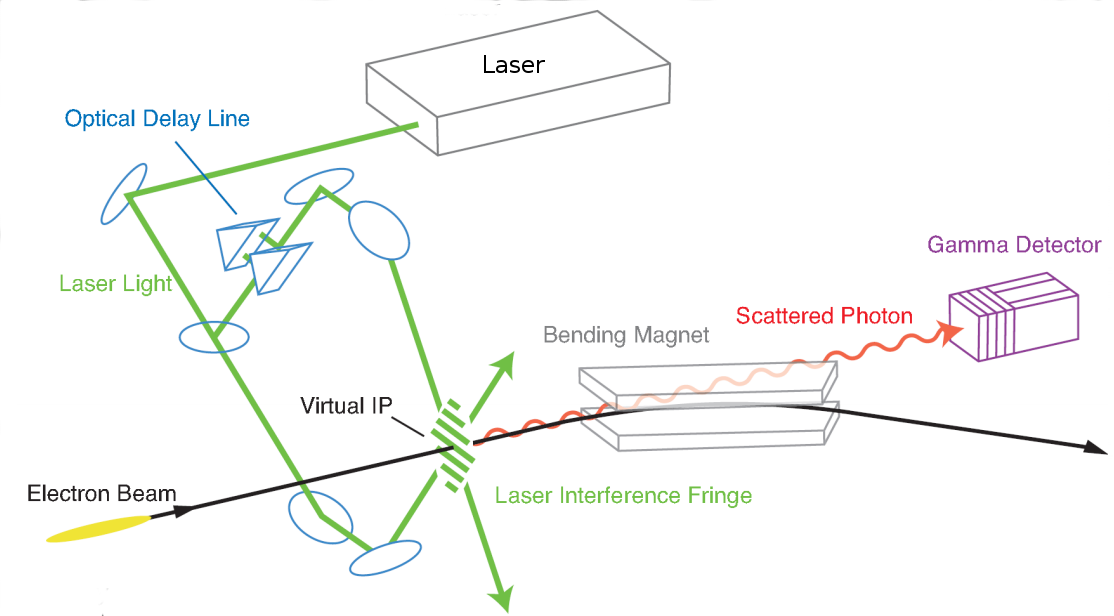
\includegraphics[angle=0,scale=0.5]{IPBSM_1.png}\caption{IPBSM schematic design. The particle beams crosses the interference pattern generated by a perpendicular beam. The number of electron-photon interactions varies with the fringe size and the particle beam size.}\label{f:IPBSM}
 \end{center}
\end{figure}
It was previously used at the FFTB line at SLAC \cite{Shintake:1995sg} and now it is located now in the IP region at ATF2 \cite{Jackelinethese}.\par
\begin{figure}[htb]
 \begin{center}
  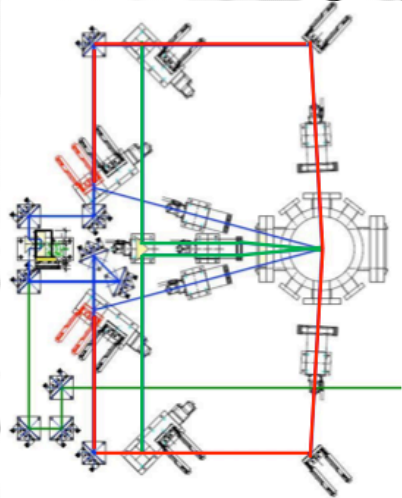
\includegraphics[angle=0,scale=0.35]{IPBSM_angles.png}
  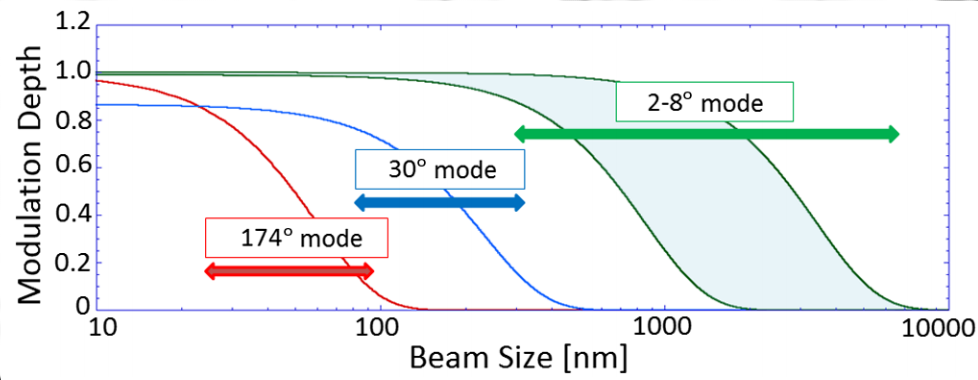
\includegraphics[angle=0,scale=0.455]{IPBSMreso.png}
  \caption{(Right) IPBSM laser path over the optical table perpendicular to the beam propagation. (Left) Beam size resolution for the angle modes : $2\sim8$\degree in green, 30\degree in blue and 174\degree in red.}\label{f:IPBSMangles}
 \end{center}
\end{figure}
At ATF2, it is installed in a vertical optical table where the laser incident angle can be adjusted to change the interference fringe size measuring beam sizes from 6 $\mu$m down to 25 nm. Figure \ref{f:IPBSMangles} shows the beam path along the vertical optical table for three angles modes and the correspoding range of beam measurements.\par
Larger beam sizes are measured by a wire scanner installed in the same region. It consists in a wire moved across the beam generating bremstrahlung gamma rays. The number of photons is proportional to the charge of the slice interacting with the wire at each position setting. Profile is constructed from the number of photons as a function of wire position \cite{Hayano:2000xf}.

\section{Recent achievements and current work}
In 2014 vertical beam size about 55nm was observed at ATF2 \cite{Kubo50nm}, and since then smaller beam size can be achieved systematically down to 44nm \cite{KuboCLICws2015} demonstrating the local chromaticity correction method at charges below $0.1\times10^{10}$ particules per bunch.\par
The identified issue of intensity dependence is currently explored by the ATF2 collaboration. However, at low intensities the beam size remains above the designed 37nm. Possible contributions are: (1) the increase of the incoming beam emittance through out the ATF2 line, (2) systematic errors and resolution limitations on the beam size monitor, (3) beam drift beyond the tolerable margin and  (4) undetected optics mismatch.\par
Last two issues can be adressed by measuring the beam trajectory in the IP Region after the Final Doublet. In adittion, looking forward to \textbf{goal 2}, beam position measurement is a requirement for beam stabilization.\par
The work here described corresponds to the beam position monitors installed in 2013 by LAL in collaboration with Kyungpook National University (KNU), the Feedback in Nanosecond Timescale (FONT) group from Oxford, and the ATF2 staff.\par